\documentclass[../../relatorio.tex]{subfiles}
\begin{document}
Neste subsistema podem-se encontrar as funcionalidades relacionadas com os \textbf{Clientes}. 
Apesar de cada subsistema não estar intrinsecamente dependente de outros, estes não deixam de 
se relacionarem, como se pode verificar neste caso, com o SSReparacoes. Também é de salientar que neste
subsistema predomina uma arquitetura com agregação entre classes.


Aqui encontra-se, entre a classe Equipamento e Cliente, um caso de navegabilidade bidirecional, 
na medida a facilitar o acesso. É de salientar a atribuição de um estado ao equipamento, de maneira, a facilitar todo o processo da reparação, 
atribuíndo um ponto de situação ao mesmo e, também, a atribuição de uma forma de contacto ao cliente, de maneira a que este possa ser contactado quando necessário.


\subsubsection{GestClientesFacade}
Esta classe permite a gestão dos clientes e dos respetivos equipamentos associados, implementando a interface IGestClientes.

Analisando os métodos que esta classe implementa, identificou-se que, para melhorar a navegabilidade
e a \textit{performance} do sistema, será necessário que este tenha um conjunto de atributos, nomeadamente:
\begin{itemize}
    \item[clientes]{Mapa de clientes que pode ser acessido através do seu identificador, nif}
    \item[equipamentos]{Mapa de equipamentos que pode ser acessido através do seu ID} 
\end{itemize}

\begin{figure}[!ht]
    \centering
    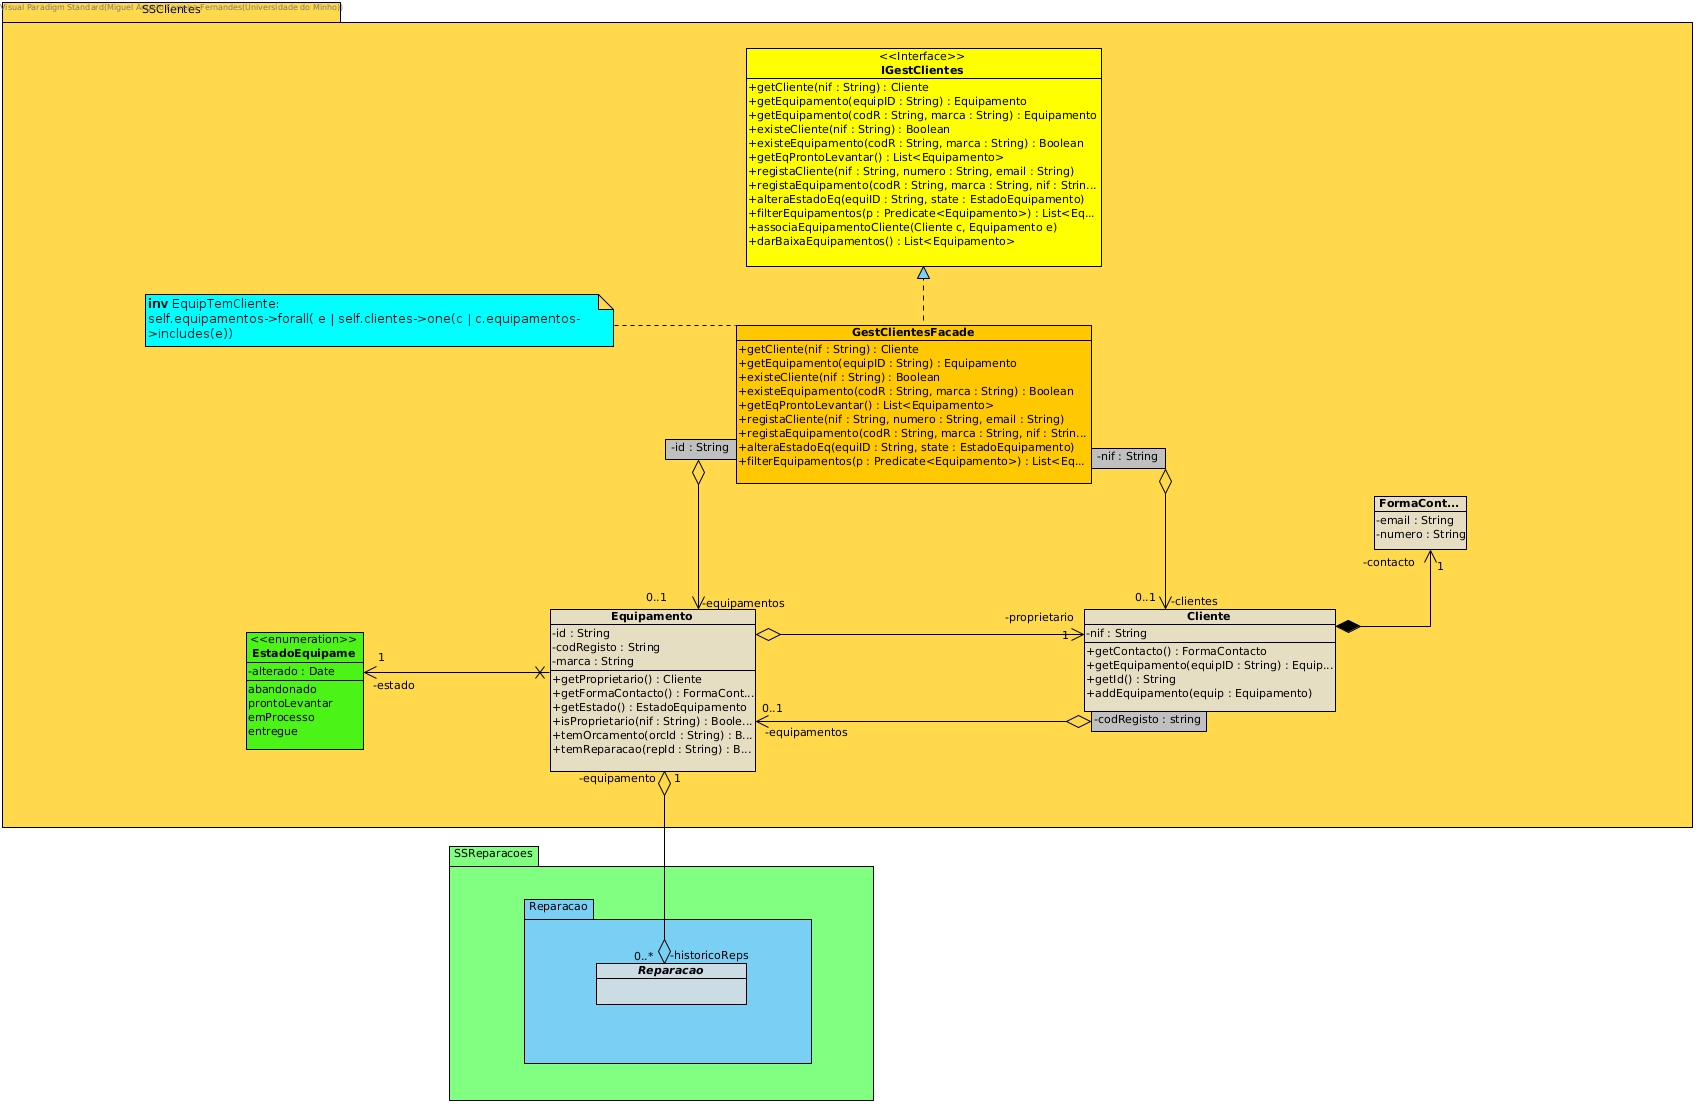
\includegraphics[scale=0.29]{SSClientes.jpg}
    \caption{SubSistema SSClientes}
\end{figure}
\end{document}